\chapter{Linguistic structures}
\label{ch:chapter4}


\ex. \begin{minipage}[t]{.4\textwidth}
\textbf{Constituent structure:} \\
\Tree [.IP [.NP Jordan  ]  [.I$'$ [.VP [.V visited ] [.NP Alex ] ] ] ]
    \end{minipage}%
    \begin{minipage}[t]{.5\textwidth}
     \textbf{Semantics:} \\
       \begin{center}
         	\begin{prooftree}
		\AxiomC{$\lambda x. \lambda y.\text{visit}(y,x): g \multimap (h \multimap f)$}
		\AxiomC{$a : g$}
		%\RightLabel{$\multimap_{E}$}
		\BinaryInfC{$\lambda y.\text{visit}(y,a): h \multimap f$}
		    \AxiomC{$j : h$}	
\BinaryInfC{$\text{visit}(j,a): f$}
	\end{prooftree}
    \end{center}
    \end{minipage} \\%
    \hspace*{\fill}\\ 
    \begin{minipage}[t]{.4\textwidth}
    \textbf{Functional structure:} \\
    \hspace*{\fill}\\ 
    \begin{avm}
     \[ \avmspan{PRED `$<$Jordan, Alex$>$'} \\
        SUBJ & \[ PRED `Jordan' \] \\
        OBJ & \[ PRED `Alex' \] \\ 
        TENSE past \]
    \end{avm}
    \end{minipage}%
    \begin{minipage}[t]{.5\textwidth}
    \textbf{Discourse representation/model:}\\%
    \hspace*{\fill}\\
    \drs{e,x,y,t,n}{visit(e) \\ ag(e) = x \\ th(e) = y \\ x = Jordan  \\ y = Alex \\ e $\subseteq$ t \\ t $\prec$ n }
    \end{minipage}%


\section{Trees}

%Tree drawn with qtree syntax
\ex. \Tree [.IP [.NP Jordan ] [.I$'$ [.VP$_{[fin]}$ [.V seems ] [.CP [.C$'$  [.C to ] [.VP$_{[inf]}$ [.V like ] [.NP Alex ] ] ] ] ] ] ]

%Tikz-qtree version with additional options
\begin{figure}[!h]
\begin{center}
\begin{tikzpicture}
\Tree [.AP 
    [.A \edge[roof]; {tall +comp} ] 
    [.CP 
        [.C than ] 
        [.NP \edge[roof]; {the cat} ]
    ] 
]
\end{tikzpicture}
\end{center}
\caption{Often trees are best treated as figures}
\end{figure}

\ex. \begin{dependency}
\begin{deptext}
John \& kissed \& a \& girl \\
NNP/1 \& VBD/2 \& DET/3 \& NP/4 \\
% \& Tense=past \& \\
% \& VerbForm=fin \& \\
\end{deptext}
\depedge{2}{4}{obj}
\depedge{3}{4}{det}
\depedge{2}{1}{nsubj}
\deproot{2}{root}
\end{dependency}

\begin{footnotesize}

\begin{tikzpicture}
    \tikzset{every tree node/.style={align=center,anchor=north}}
\tikzset{grow'=up}
\tikzset{level 1+/.style={level distance=30pt}}
\tikzset{frontier/.style={distance from root=180pt}}
\Tree 
[.{FA}
                [.{FA} 
                    [.{} \node(14){$s_t \multimap f_t \multimap f_t$\\14}; ] 
                    [.{FA} 
                        [.{} \node(15){$s_e \multimap s_t$\\15}; ] 
                        [.{} \node(18){$s_e$\\18}; ] 
                    ] 
                ] 
    [.{FA}
                [.{FA} 
                    [.{} \node(16){$g_t \multimap f_t \multimap f_t$\\16}; ] 
                    [.{FA} 
                        [.{} \node(17){$g_e \multimap g_t$\\17}; ] 
                        [.{} \node(20){$g_e$\\20}; ] 
                    ] 
            ]
                [.{FA} 
    [.{FA} 
        [.{FA} 
                [.{} \node(13){$h_e \multimap s_e \multimap g_e \multimap f_t$\\13}; ]  
                  [.{} \node(12){$h_e$\\12}; ] 
            ]
             [.{} \node(19){$s_e$\\19}; ] 
            ]
            [.{} \node(21){$g_e$\\21}; ] 
            ]
        ] 
    ]
\end{tikzpicture}
\end{footnotesize}

\section{Fancy examples}

Projection architecture:

\begin{minipage}[t]{.3\textwidth}
\Tree [.{\tikznode{snor}{S}} [.{\tikznode{vpnor}{VP}} 
[.V {Joi-\textcircled{n}} ] 
[.{\tikznode{npnor}{NP}} kahvia ] ]  ]
\end{minipage}%
\begin{minipage}[t]{.5\textwidth}
\begin{avm}
{{\tikznode{fstrnor}{$f$}}}\[ \avmspan{PRED `drink$<$pro,coffee$>$'} \\
OBJ & {{\tikznode{fstrobjnor}{$h$}}}\[PRED `coffee' \\
NUM sg \\ PERS 3 \\ CASE partitive \] \\
SUBJ & {{\tikznode{fstrsubjnor}{$g$}}}\[PRED `pro' \\
NUM sg \\ PERS 1 \] \\
\avmspan{TENSE past}
\]
\end{avm}
\end{minipage}
\begin{tikzpicture}[overlay, remember picture]

    % Manual node placement (Corresponding to the left daughters of the tree)
    \node[overlay] at (-9.2,-3.05) (morphnor) {}; % Adjust coordinates as needed
    \node[overlay] at (-9.5,-2) (vnor) {}; % Adjust coordinates as needed

    % Arrow from c1 to c1s
\draw[->, bend right=10, looseness=1,-latex] 
    (snor) to [out=20, in=190] 
         (fstrnor.west);

\draw[->, bend right=10, looseness=1,-latex] 
    (vpnor) to [out=20, in=180] 
         (fstrnor.west);

\draw[->, bend right=10, looseness=1,-latex] 
    (vnor) to [out=30, in=165] 
         (fstrnor.west);

    \draw[->, bend right=5, looseness=0.9,-latex] 
        (npnor) to [out=330, in=220] 
             (fstrobjnor);

        \draw[->, bend right=5, looseness=0.9,-latex] 
        (morphnor) to [out=330, in=220] 
             (fstrsubjnor);    
\end{tikzpicture}\\
\strut \hfill{(based on \citealt{toivonen2023pronoun}: ex.~(6))} \\





\begin{figure}[!h]
\centering
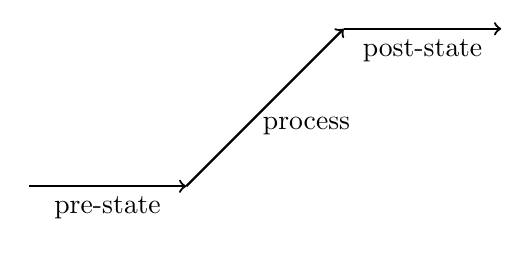
\begin{tikzpicture}
   \tkzInit[xmax=6,ymax=4,xmin=0,ymin=0]%
   %\tkzGrid
   %\tkzAxeXY
    \tkzSetUpAxis[ticka=0pt, tickb=0pt]
   \tkzDrawX[label=t] \tkzDrawY[label=q]
  % \draw[->, thick] (0,2) -- (2,2) node[below]{post-state};
   \draw[->, thick] (0,1) -- node[below]{pre-state} ++(2,0);
   \draw[->, thick] (4,3) -- node[below]{post-state} ++(2,0);
      \draw[->, thick] (2,1) -- node[below]{\quad\quad\quad process} ++(2,2);
%   \draw[->, thick] (2,2) -- (4,6) node[above]{process};
%\draw[->, thick] (4,6) -- (6,6) node[below]{pre-state};

   % two points for drawing 2x+y=2
   %\tkzText[above](0,6.75){Desired Output}
  \end{tikzpicture}
  \caption{A diagram describing the temporal progression of an event}
  \label{ch4:fig:inner-asp-2d}
\end{figure}



\newpage
For typsetting movement-analyses, I manually position nodes, because somehow tikz struggles with nodes defined in the left branch of a tree. 

\ex. A rudimentary X$'$-analysis for minimalists \\
 \begin{minipage}[t]{.5\textwidth}
 $\approx$\textit{The chicken can start eating.} \\
 \Tree [.IP [.NP \edge[roof]; {the chicken$_1$} ] [.I$'$ [.I is ] [.VP [.AP ready ] [.CP [.{$t_1$} ] [.C$'$ [.C to ] [.VP eat ] ] ] ] ] ] 
\end{minipage}%
\begin{minipage}[t]{.5\textwidth}
 $\approx$\textit{The chicken is ready to be eaten.} \\
 \Tree [.IP [.NP \edge[roof]; {the chicken$_2$} ] [.I$'$ [.I is ] [.VP [.AP ready ] [.CP [.\textsc{pro} ] [.C$'$ [.C to ] [.VP [.V eat ] [.{\tikznode{readysyntrace2}{$t_2$}} ] ] ] ] ] ] ]
\end{minipage}
\begin{tikzpicture}[overlay, remember picture]
    % Manual node placement
    \node[overlay] at (7.7,5.5) (readysynp2) {}; % Adjust coordinates as needed
    \node[overlay] at (4.4,3.3) (readysyntrace1) {}; % Adjust coordinates as needed
        \node[overlay] at (1.3,5.5) (readysynp1) {}; % Adjust coordinates as needed
    % Arrow from c1 to c1s
    \draw[->, dashed, bend right=5, looseness=1] 
        (readysyntrace1) to [out=120, in=130] 
             (readysynp1); 
    % Arrow from c2 to c2s
    \draw[->, dashed, bend right=5, looseness=1.5] 
        (readysyntrace2) to [out=120, in=130]
          (readysynp2);
\end{tikzpicture}
  



